%
%  kant.four
%
%  Created by Mark Eli Kalderon on 2007-08-05.
%  Copyright (c) 2007 Mark Eli Kalderon. All rights reserved.
%
%  Beamer

% Definitions and macros
\newcommand{\change}{\textcolor{blue}{\textbf{CHANGE SLIDE}}}
\newcommand\myauthor{Mark Eli Kalderon} 
\newcommand\mytitle{Introduction to Moral Philosophy}
\newcommand\mysubtitle{Kant}
\newcommand\myinstitution{University College London}
\newcommand\myurl{http://markelikalderon.com/teaching/}

% Packages specific to lecture notes
\mode<article>{
	\usepackage{palatino}
}

% Packages specific to beamer presentation
\mode<presentation>{
	\usetheme{Darmstadt}
	\setbeamercovered{transparent}
	\pgfdeclareimage[height=0.5cm]{university-logo}{../../graphics/logo_sml_blk}
	\logo{\pgfuseimage{university-logo}}
}

% Packages common to lecture notes and beamer presentation
\usepackage{pgf}
\usepackage{tikz}
\usepackage{hyperref}

\setjobnamebeamerversion{kant.four.beamer}

\title{\mytitle}
\subtitle{\mysubtitle} % (optional)

\author{\myauthor\\
\url{\myurl}}
\institute{\myinstitution}

% \date[Short Occasion] % (optional)
% {Date / Occasion}

\begin{document}

\frame{\maketitle}

\section{Review From Last Time}\label{sec:review_from_last_time} % (fold)

\change\ Last time, we began discussing the second section. In the second section, Kant characterizes the supreme principle of morality in terms of a system of three formulas. We began discussing the First Formula with special attention to one of its variant formulations, The Formula of Law of Nature. We apply the Formula of the Law of Nature to determine the moral permissibility of a a \emph{maxim}, a policy that we implicilty adopt whenever we act. The first step in applying the Formula of Law of Nature is to specify the maxim to be tested. It will be roughly of the form:
\begin{quote}
    I am to perform action A in circumstances C in order to bring about end E.
\end{quote}
The second step is to generalize the maxim so that it applies to everyone:
\begin{quote}
    Everyone is to perform action A in circumstances C in order to bring about end E.
\end{quote}
The third step is to transform the generalized maxim into a law of nature:
\begin{quote}
    It is a law of nature that everyone performs action A in circumstances C in order to bring about end E.
\end{quote}
The fourth step is to conjoin the hypothetical law of nature to existing laws of nature and to work out the consequences of this in determining the new system of nature:
\begin{quote}
    Conjoin the hypothetical law of nature to the laws of nature as we undertand them and work out what the system of nature would be once the effects of conjoining the novel law stabilizes.
\end{quote}
The target maxim is permissible just in case one an coherently will the resulting system of nature. Kant distinguishes two tests for whether a person can coherently will the hypothetical system of nature:
\begin{enumerate}
    \item \emph{Contradiction in Conception}: The hypothetical system of nature cannot be conceived without self-contradiction.
    \item \emph{Contradiction in Volition}: They hypothetical system of nature cannot be willed without contradicotry volition.
\end{enumerate}

We saw, for Kant, these tests mark a morally significant distinction: Maxims that violate the contradiction in conception test violate \emph{perfect} duties; whereas maxims that violate the contradiction in volition test violate \emph{imperfect} duties. Perfect duties admit of no exception in favor of inclination whereas imperfect duties do. In \emph{The Metaphysics of Morals}, Kant explains further. \emph{Perfect duties} are requirements on actions and any violation of a perfect duty is an instance of wrongdoing and hence blameworthy. \emph{Imperfect duties} are requirements on the adoption of ends though there is latitude in the fulfillment of these ends since a person has a variety of ends and these must be rationally ordered. (This is the sense in which they admit of exception in favor of inclination.) Specific actions taken toward the fulfillment of required ends is meritorious, whereas the failure to act toward the fulfillment of the required end merely lacks merit and is not an instance of wrongdoing and hence not blameworthy. \change

\begin{frame}<presentation>[label=slide1]
    \frametitle{Review from Last Time}
        \begin{enumerate}
            \item I am to perform action A in circumstances C in order to bring about end E.
            \item Everyone is to perform action A in circumstances C in order to bring about end E.
            \item It is a law of nature that everyone performs action A in circumstances C in order to bring about end E.
            \item  Conjoin the hypothetical law of nature to the laws of nature as we undertand them and work out what the system of nature would be once the effects of conjoining the novel law stabilizes.
        \end{enumerate}
\end{frame}

% section review_from_last_time (end)

\section{Problems with the First Formula}\label{sec:problems_with_the_first_formula} % (fold)

There are two potential problems for the application of the Formula of the Law of Nature: First, applying the formula may classify morally impermissible maxims as permissible; second, applying the formula may classify morally permissible maxims as impermissible. If the proper application of the Formula of the Law of Nature classifies morally impermissible maxims as permissible, then passing the univeralizability test is not sufficient for a maxim to be permissible. If the proper application of the Formula of the Law of Nature classifies morally permissible maxims as impermissible, then passing the universalizability test is not necessary for a maxim to be permissible. \change

Many commentators (Hegel, Mill, and Sidgwick among them) have criticized the Formula of the Law of Nature on the grounds that it improperly classifies immoral maxims as morally permissible. If such maxims exist, then passing the universalizabilty test is not sufficient for a maxim to be morally permissible.

To see how there could be such maxims, first consider how maxims differ in degree of generality or specificity. Some maxims such as:
\begin{quote}
	\ldots when I believe myself to be in need of money I shall borrow money and promise to repay it, even though I know that this will never happen. (G 4:422)
\end{quote}
are more general than other maxims:
\begin{quote}
	When I believe myself to be in need of money I shall borrow money from Jones on the second Tuesday of the Month and promise to repay it, even though I know that this will never happen.
\end{quote}

The latter maxim is more specific than the former more general maxim in the sense that it restricts the conditions under which the false promise would be made.

Second, just as maxims can differ in their degree of specificity so can the hypothetical laws of nature that correspond to them. Moreover, the greater the specificity of the law the less widespread its effects would be. The effects of conjoining a more specific hypothetical law to the existing laws of nature would be less widespread than the effects of conjoining a more general law. Thus while the effect of making false promises when in need of money a law of nature would be that no promise would be believed, the effects of making false promises to Jones on the second Tuesday of every month a law of nature would be less widespread. Perhaps people named Jones would fail to believe promises made on the second Tuesday of the month especially if made by people known to be in debt, but promises would otherwise be believed. Since promises would be believed in general (except by some in exceptional circumstances) this would be consistent with the possibility of promising. And if promising is possible in the resulting system of nature then, for all Kant has said, it is conceivable without self-contradiction. Thus, an immoral maxim, to make false promises to Jones on the second Tuesday of the month, passes the universalizabilty test. So passing the universalizability test is not sufficient for a maxim to be morally permissible. \change

The Formula of the Law of Nature can be criticized on the grounds that it improperly classifies morally permissible maxims as impermissible. To see how there could be such maxims, consider innocuous actions whose existence depends on their being exceptional. There is nothing immoral about adopting the following financial policy: I will sell my stocks when the Dow hits 10,000.

But the policy would lack the financial benefits that it actually has in a world where it is a law of nature that everyone sells their stock when the Dow hits 10,000. If everyone is selling, who is there to buy? And if no one is buying, the selling of stock is not possible under those circumstances. But that means that the resulting system of nature cannot be conceived without self-contradiction. Thus a morally permissible maxim, to sell stock when the Dow hits 10,000, fails the universalizability test. So passing the universalizabilty test is not necessary for a maxim to be morally permissible. \change

\begin{frame}<presentation>[label=slide2]
    \frametitle{Problems with the First Formula}
        \begin{itemize}
            \item<2-> \alert{Failures of Sufficiency}: The Formula of Law of Nature improperly classifies immoral maxims as permissible. If there are such maxims, then the universalizability test is not sufficient for a maxim to be permissible
           \item<3-> \alert{Failures of Necessity}: The Formula of Law of Nature improperly classifies morally permissible maxims as impermissible. If there are such maxims, then the unversalizability test is not necessary for a maxim to be permissible.
        \end{itemize}
\end{frame}

Applying the Formula of the Law of Nature fails to provide a test the satisfaction of which is both necessary and sufficient for a maxim to be permissible. Or at least, at this stage of the Groundwork, our understanding of the first formula is subject to these failures. Recall, the three formulas are supposed to represent different aspects of the same law. This places a constraint on our interpretation of them: Each should be interpreted in light of the other. Perhaps when the Formula of the Law of Nature is interpreted in light of the other formulas, the failures of necessity and sufficiency will be avoided. Indeed, Kant discusses the four examples again in light of the Formula of Humanity. His case for the impermissibility of these maxims is deepened and illuminates and supports his earlier arguments. So one possibility is that the failures of necessity and sufficiency are due to an incomplete understanding of the Formula of the Law of Nature.

Even so, perhaps the Formula of the Law of Nature was never intended to be a mechanical algorithm for determining the permissibility of maxims. When Kant claimed that the first formula is a ``compass'' sufficient for common rational moral cognition to act in conformity with duty, perhaps he did not promise a test the satisfaction of which is necessary and sufficient for the permissibility of a given maxim. Even if they were possible, no such test would be mechanical. The application of the Formula of the Law of Nature not only requires background empirical information but judgement as to its relevance as well.

If the first formula is not an algorithm for determining the permissibility of maxims, in what sense is it a moral compass?

What’s the moral point of the first formula? Kant provides an explicit answer:

\begin{quote}
	If we now attend to ourselves in any transgression of duty, we find that we do not really will that our maxim should become a universal law, since that is impossible for us, but that the opposite of our maxim should instead remain a universal law, only we take the liberty of making an exception to it for ourselves (or just for this once) to the advantage of our inclination. Consequently, if we weighed all cases from one and the same point of view, namely that of reason, we would find a contradiction in our own will, namely that a certain principle be objectively necessary as a universal law and yet subjectively not hold universally but allow exceptions. (G 4:424)
\end{quote}

Normally, when we act contrary to duty, we will “that the opposite of our maxim should instead remain a universal law, only we take the liberty of making an exception to it for ourselves (or just for this once) to the advantage of our inclination.” When tempted to make false promises when in need of money, we do not will that everyone should make false promises when in need of money. Rather if we succumb to temptation, we will that in general people truly promise only that we, just this once, falsely promise to repay a creditor. In acting contrary to duty, a person gives unjustifiable preference to his own inclinations over the inclinations of other finite rational beings.

It is the counterweight of inclination that tempts otherwise innocent human beings to act contrary to duty. Specifically, human beings possess:

\begin{quote}
	\ldots a propensity to rationalize against those strict laws of duty and to cast doubt upon their validity, or at least upon their purity and strictness, and where possible, to make them better suited to our wishes and inclinations, that is, to corrupt them at their basis and to destroy all their dignity---something that even common rational cognition cannot, in the end, call good. (G 4:405)
\end{quote}

Perhaps the first formula is a moral compass for those lost to temptation in the following sense: It is a reminder not to make oneself a special exception to a moral law that everyone else must follow. Perhaps the moral point of the first formula is as a vivid reminder not to give unjustified preference to ones own inclinations over the inclinations of other finite rational beings, and hence as a corrective to our human propensity to make exceptions for ourselves. \change

\begin{frame}<presentation>[label=slide3]
    \frametitle{The Moral Point of the First Formula}
        \begin{columns}
            \begin{column}{3cm}
                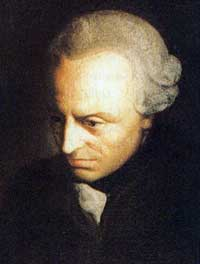
\includegraphics[height=4cm]{../../graphics/kant.jpg}
            \end{column}
            \begin{column}{7cm}
                \alert{The moral point of the first formula is as a vivid reminder not to give unjustifed preference to ones own inclinations over the inclinations of other finite rational beings, and hence as a corrective to our human propensity to make exceptions for ourselves.} 
            \end{column}
        \end{columns}
\end{frame}

% section problems_with_the_first_formula (end)

\section{The Second Formula}\label{sec:the_second_formula} % (fold)

Whereas the first formula of the supreme principle of morality specifies the form of the moral law---its validity for all rational beings, the second formula specifies its matter (G 4:436)---the end involved in acting on a law valid for all rational beings:
\begin{quote}
    \emph{The Formula of Humanity}: ``So act that you use humanity, whether in your own person or in the person of any other, always at the same time as an end, never merely as a means.'' (G 4:429; 4:436)
\end{quote}

\change

\begin{frame}<presentation>[label=slide4]
    \frametitle{The Formula of Humanity}
        \begin{columns}
            \begin{column}{3cm}
                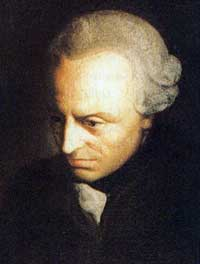
\includegraphics[height=4cm]{../../graphics/kant.jpg}
            \end{column}
            \begin{column}{7cm}
                ``So act that you use humanity, whether in your own person or in the person of any other, always at the same time as an end, never merely as a means.'' (G 4:429; 4:436)
            \end{column}
        \end{columns}
\end{frame}

Ends are that for the sake of which we act. Kant distinguishes between two kinds of ends:
\begin{itemize}
\item \emph{Objective ends}, i.e., ends given by reason alone that are valid for all rational beings;
\item \emph{Subjective ends}, i.e., ends given by inclination that can vary from one rational being to another.
\end{itemize}

Kant calls objective ends ``motives'' and subjective ends ``incentives''. Every action has end: We always act for the sake of some end or another. So in acting from duty we act for the sake of some end. Since the moral law is valid for all rational beings the end involved in acting from duty must be an objective end or motive.

When Kant describes the nature of motives, he is providing additional information about what it means to act from duty. In the first section, Kant characterized acting from duty as acting from respect for the moral law. Respect for the law was so far conceived to merely be to the determination of the will by a law valid for all rational beings and consciousness of this. This, however, only describes the ``form'' of the law but not its ``matter''. In the first section, Kant remarks that he ``does not yet see what this respect is based upon (this the philosopher may investigate)'' (G 4:403). Kant is now conducting just this philosophical investigation. In describing the nature of motives, Kant is describing the end involved in acting from duty that is the basis of our respect for the moral law. \change

\begin{frame}<presentation>[label=slide5]
    \frametitle{Ends and the Will}
        \begin{columns}
            \begin{column}{3cm}
                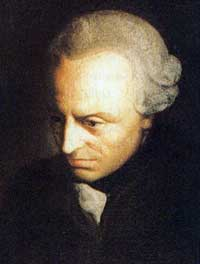
\includegraphics[height=4cm]{../../graphics/kant.jpg}
            \end{column}
            \begin{column}{7cm}
                \begin{itemize}
                    \item \alert{Objective ends}, i.e., ends given by reason alone that are valid for all rational beings;
                    \item \alert{Subjective ends}, i.e., ends given by inclination that can vary from one rational being to another.
                \end{itemize}
            \end{column}
        \end{columns}
\end{frame}

Subjective ends or incentives, ends given by inclination, have only a conditional value or worth and, hence, are ``only the grounds of hypothetical imperatives'' (G 4:428). Objective ends or motives, ends given by reason alone, have a different significance:
\begin{quote}
But suppose there were something the \emph{existence of which in itself} has an absolute worth, something which as an \emph{end in itself} could be a ground of determinate laws; then in it, and in it alone, would lie the ground of a possible categorical imperative, that is, of a practical law.
\end{quote}

Kant, in describing the nature of motives or objective ends, is supposing the existence of something that has three distinct features:
\begin{itemize}
\item It is an \emph{end in itself}
\item It is an \emph{existent end}
\item It has \emph{absolute worth}
\end{itemize}

Let’s consider these in turn. \change

First, Kant is supposing the existence of something that is an \emph{end in itself} or an \emph{objective end}. An end in itself is something whose worth is unconditional, independent of inclination, and valid for all rational beings. Kant contrasts ends in themselves with \emph{relative ends}, ends whose worth is conditional and dependent on inclination which varies from one rational being to another. Relative ends could only be incentives and, hence, could only be the grounds of hypothetical imperatives (G 4:428). \change

Second, Kant is supposing the existence of an \emph{existent end} or \emph{independently existing end} (G 4:437). An existent end is something that already exists and ``whose existence is in itself an end'' (G 4:428). Kant contrasts existent ends with **ends to be effected**. An end to be effected is something that does not yet exist but can be brought about by action (G 4:437). It is tempting to suppose that there is nothing more to the concept of an end than a state of affairs to be brought about by action. But the concept of an end is broader than that. An end is that for the sake of which we act. We can act for the sake of a state of affairs to be brought about by action but we can act for the sake of other ends as well. We can act for the sake of our self-preservation and continued well-being. These cannot be brought about by our actions but are already existing states of affairs that we merely preserve and do not act against. \change

Third, Kant is supposing the existence of something that has \emph{absolute worth}. The contrast might be with things with relative worth. So understood things with absolute value would be ends in themselves. Kant, however, might mean more than this. Kant might be supposing the existence of something with \emph{dignity}, a value that cannot be measured against the value of anything else (G 4:434). Kant contrasts dignity with \emph{price}. An end with only relative worth, or price, can be measured against the value of something else and may be sacrificed to obtain something else of equivalent or greater worth.

These three features are conceptually distinct. Thus, nonrational animals are plausibly examples of existent ends that neither have absolute value nor are ends in themselves. Nevertheless, Kant claims that there is exactly one thing that has all three features---humanity or rational nature. Indeed, Kant seems to claim that humanity is an end in itself by being an existent end with absolute worth or dignity.

At this point Kant has argued that in order for a categorical imperative to motivate the will of a rational being it must involve an end in itself as a ground of the rational will. Supposing there is such a thing as an end in itself, what could it be? Kant’s answer comes in two stages. The first stage is negative: Kant considers three kinds of things we consider to be either valuable or sources of value and argues that they are not ends in themselves. These are:
\begin{enumerate}
    \item The objects of inclination
    \item The inclinations themselves
    \item Nonrational beings whose existence does not depend on our will
\end{enumerate}
The second stage is positive: Kant argues that humanity or rational nature is an end in itself. \change

\begin{frame}<presentation>[label=slide6]
    \frametitle{Ends in Themselves}
        \begin{columns}
            \begin{column}{3cm}
                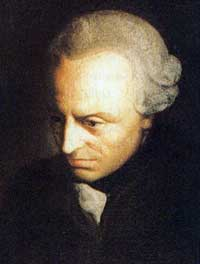
\includegraphics[height=4cm]{../../graphics/kant.jpg}
            \end{column}
            \begin{column}{7cm}
                \begin{itemize}
                \item<2-> It is an \alert{end in itself}
                \item<3-> It is an \alert{existent end}
                \item<4-> It has \alert{absolute worth}
                \end{itemize}
            \end{column}
        \end{columns}
\end{frame}

Let's begin by considering the initial negative stage of the argument where Kant considers and rejects three candidates for being ends in themselves

\emph{Objects of Inclination}. An end in itself, if it is the end involved in acting from duty, must have a worth or value valid for all rational beings. However, the objects of inclination only have value for those who are so inclined. The value of an object of inclination is contingent upon the existence of that inclination: ``All objects of the inclinations have only conditional worth; for, if there were not inclinations and the needs based on them, their object would be without worth'' (G 4:428). Since their worth depends on the existence of the relevant inclination, and these can vary from one rational being to another, objects of inclination cannot be ends in themselves. \change

\emph{Inclinations Themselves}. Kant argues that (G 4:428): ``the inclinations themselves, as sources of needs, are so far from having absolute worth, so as to make one wish to have them, that it must instead be the universal wish of every rational being to be altogether free from them.'' This is an extraordinary claim. How are we to make sense of it? Kant seems to think that the inclinations themselves are not valued simply as such any more than their objects are. Moreover, even when we do value the objects of inclination, we don’t necessarily value the inclination considered as the source of that value. That it is not irrational to wish to be altogether free of them can be understood as a hyperbolic expression of this latter claim. Kant might also be dramatically contrasting the absolute value or dignity of ends in themselves with the value of things with merely relative worth or price. Kant now infers: ``Thus the worth of any object *to be acquired* by our action is always conditional'' (G 4:428). Thus an end in itself must be an existent end. \change

\emph{Nonrational Beings}. Existent ends are pre-existing things for the sake of which we act. These might be rational beings or nonrational beings. Ends in themselves may be existing ends but these existing ends could not be nonrational beings (G 4:428):
\begin{quote}
    Beings the existence of which rests not on our will but on nature, if they are beings without reason, still have only relative worth, as means, and are therefore called \emph{things}, whereas rational beings are called \emph{persons} because their nature already marks them out as an end in itself, that is, as something that may not be used merely as a means, and hence so far limits all choice (and is an object of respect).
\end{quote}
This is unconvincing. The ordinary distinction between persons and things may presuppose that things are of lesser value than persons but it does not obviously commit us to valuing them *merely as means*. However, Kant might be anticipating the positive argument from which this might be derived as a consequence. \change

\begin{frame}<presentation>[label=slide7]
    \frametitle{The Negative Argument}
        \begin{enumerate}
            \item<1-> The objects of inclination
            \item<2-> The inclinations themselves
            \item<3-> Nonrational beings whose existence does not depend on our will
        \end{enumerate}
\end{frame}

If the objects of inclination, the inclinations themselves, and nonrational beings whose existence does not depend on our will are not ends in themselves, then what is? We know that ends in themselves must be existent ends but cannot be nonrational beings, so an existent end that is an end in itself must at least inhere in rational beings. Specifically, it must be humanity or rational nature. While Kant cannot demonstrate this, he argues that we necessarily, if implicitly, presuppose this. Kant’s positive argument has four steps:

\begin{quote}
	The ground of this principle is: \emph{rational nature exists as an end in itself}. (1) The human being necessarily represents his own existence in this way; so far it is thus a \emph{subjective} principle of human actions. (2) But every other rational being also represents his existence in this way consequent on just the same rational ground that also holds for me; (3) thus it is at the same time an objective principle from which, as a supreme practical ground, it must be possible to derive all laws of the will. (4) The practical imperative will therefore be the following: \emph{So act that you use humanity, whether in your own person or in the person of any other, always at the same time as an end, never merely as a means}.
\end{quote}

(1) cannot be read as a contingent empirical claim about how people explicitly value their own existence for so interpreted it would be false---unfortunately some people regard their existence as being without worth. So how are we to understand (1)? According to Kant, our humanity or rational nature consists, at least in part, in our capacity to set ends (G 4:437). Given this, Kant might be understood as claiming that when we value the ends we set for ourselves, we must, \emph{implicitly} at least, value our capacity to set these ends (whether or not we \emph{explicitly} value this capacity in our own person). If we didn’t, what confidence could we have on the value we place on these ends? Our capacity to set ends is an existent end whose value is unconditional---at least it does not depend on the ends we set or on our inclinations. Moreover the capacity to set ends is confined to rational beings. So far, humanity is a good candidate for being an end in itself. But before he can conclude that it is, Kant must establish that humanity has a worth or value valid for all rational beings. This is why, at this point, he merely describes himself as establishing a ``subjective principle of human action''. However, our rational nature is a nature that we share with other rational beings. Thus (2) claims that every rational being also represents its own existence as an end in itself ``on just the same rational ground'' that holds for every other rational being, i.e., their rational nature. So we must understand the value of rational nature as an objective value, valid for all rational beings. So as (3) claims, all rational beings are ends in themselves and this makes an objective claim on all rational beings to recognize themselves and others as ends in themselves. This leads to (4): the formulation of the categorical imperative as the requirement to use humanity in every rational being always as an end and never only as a means. \change

\begin{frame}<presentation>[label=slide8]
    \frametitle{The Positive Argument}
        The ground of this principle is: \alert{rational nature exists as an end in itself}.
        \begin{enumerate}
            \item The human being necessarily represents his own existence in this way; so far it is thus a \alert{subjective} principle of human actions. 
            \item But every other rational being also represents his existence in this way consequent on just the same rational ground that also holds for me;
            \item thus it is at the same time an \alert{objective} principle from which, as a supreme practical ground, it must be possible to derive all laws of the will.
            \item The practical imperative will therefore be the following: \alert{So act that you use humanity, whether in your own person or in the person of any other, always at the same time as an end, never merely as a means}.
        \end{enumerate}
\end{frame}

% section the_second_formula (end)

\section{Applying the Formula of Humanity}\label{sec:applying_the_formula_of_humanity} % (fold)

What the Formula of Humanity demands of our actions is that they express proper respect for the dignity of humanity. It thus postulates an expressive reason for doing things. This kind of reason is familiar from everyday life. Very often it is the expressive meaning of an action that constitutes at least part of the reason for performing that action. Thus saying ``thank you'' expresses gratitude, and this is part of the reason we thank people. This kind of reason motivates people to salute the flag or make a rude remark. So the formula of humanity requires that we treat humanity as an end an never merely as a means in order to express respect for the dignity of humanity.

Notice the Formula of Humanity does not forbid our using another person as a means. When you buy a stamp from a postal clerk you are using the postal clerk as a means for acquiring that stamp despite the clerk’s evident humanity, but there is nothing morally amiss in this. Rather what is forbidden is omitting to treat a person ``at the same time as an end''. Thus the injunction to treat people ``never merely as a means'' is redundant: The moral content of the Formula of Humanity consists entirely in the injunction to treat people as ends.

So why emphasize that one should never treat people \emph{merely as a means}? The empahsis can be interpreted as a rhetorical response to a diagnosis of human wrongdoing. Human beings have a tendency to act contrary to duty, not because they altogether fail to value humanity, but because they misconceive the kind of value it has. Thus, as human beings, we have a tendency to place greater value on the objects of inclination, which merely have a ``price'' or ``relative worth'', over the value of humanity, which has instead a ``dignity'' or ``absolute worth''. This both complements and illuminates the moral point of the first formula. Kant observes that normally, when we act contrary to duty, we will ``that the opposite of our maxim should instead remain a universal law, only we take the liberty of making an exception to it for ourselves (or just for this once) to the advantage of our inclination'' (G 4:424). So in acting contrary to duty, a person gives unjustifiable preference to his own inclinations over the inclinations of other finite rational beings. Notice that, when we make an exception for ourselves, we fail to express proper respect for the dignity of humanity in ourselves or in the person of others. Indeed, Kant anticipates this explicit connection when in the first section he observes that human beings possess:
\begin{quote}
	\ldots a propensity to rationalize aginst those strict laws of duty and to cast doubt upon their validity, or at least upon their purity and strictness, and where possible, to make them better suited to our wishes and inclinations, that is, to corrupt them at their basis and to destroy all their \emph{dignity} [my emphasis]---something that even common rational cognition cannot, in the end, call good. (G 4:405)
\end{quote}

In making an exception for ourselves, we sacrifice the dignity of humanity in the person of another for a mere price and, hence, fail to properly respect that dignity. \change

\begin{frame}<presentation>[label=slide9]
    \frametitle{The Second Formula}
        \begin{columns}
            \begin{column}{3cm}
                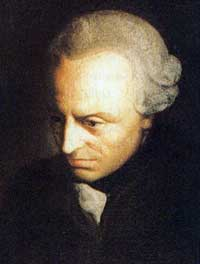
\includegraphics[height=4cm]{../../graphics/kant.jpg}
            \end{column}
            \begin{column}{7cm}
                \alert{The Formula of Humanity}: ``So act that you use humanity, whether in your own person or that of another, always at the same time as an eend, never merely as a means.'' (G 4:429; 4:436)
            \end{column}
        \end{columns}
\end{frame}

% section applying_the_formula_of_humanity (end)


The general duty not to commit suicide is derived from the expressive meaning of the act itself which Kant holds to be ``degrading to the humanity in one’s own person'' (Ms 6:422-3). In taking one’s life one fails to respect the dignity of one’s own humanity for one exhanges it for the price of maintaining ``a tolerable condition up to the end of life'' (G 4:429).

This deepens the case against suicide made on the basis of the first formula. Recall, Kant argued that since self-love has the natural function of furthering life, it is self-contradictory to suppose that there could be a system of nature that includes a law that under circumstances of more troubles than agreeableness self-love endeavors to shorten life. In the *Metaphysics of Morals*, Kant argues that we should respect the natural functions of our instinctive drives since they belong to the predisposition to animality that underpins our rational nature. Hence to use instinctive drives contrary to their natural function is to show disrespect for the humanity in one’s own person. The argument against suicide is not so much based on whether the maxim passes the contradiction in conception test as it is based on an appeal to treat self-love with proper respect for its natural function (where the basis of the appeal is the dignity of the humanity that this function underpins). \change

\begin{frame}<presentation>[label=slide10]
    \frametitle{Suicide}
        \begin{columns}
            \begin{column}{3cm}
                
\includegraphics[height=4cm]{../../graphics/suicide.jpg}
            \end{column}
            \begin{column}{7cm}
                ``If he destroys himself in order to escape from a trying condition he makes use of a person merely as a means to maintain a tolerable condition up to the end of life.'' (G 4:429)
            \end{column}
        \end{columns}
\end{frame}

We have a duty not to make promises that we do not intend to keep since making such promises treats those we deceive merely as a means for our own ends ``without taking into consideration that, as rational beings, they must always be valued at the same time as ends'' (G 4:430). The ground of this duty is the failure of our act to express respect for the humanity in the person lied to. The false promiser:
\begin{quote}
	\ldots wants to make use of another human being merely as a means, without the other at the same time containing in himself the end. For, he whom I want to use for my purposes by such a promise cannot possibly agree to my way of behaving toward him, and so himself contain the end of this action. (G 4:429--30)
\end{quote}

The deepens the case against false promises made on the basis of the first formula. If the giving and accepting of promises requires that promiser and promisee share their ends, then it is clear why promising would be impossible if it were a universal law of nature that everyone makes false promises when in need of money since this would preclude such sharing. Even making falses promises to Jones on the second Tuesday of the month would be precluded on this basis. Doing so would fail to respect the dignity of Jones’ humanity. \change

\begin{frame}<presentation>[label=slide11]
    \frametitle{False Promises}
        \begin{columns}
            \begin{column}{4cm}
                
\includegraphics[height=4cm]{../../graphics/false_promises.jpg}
            \end{column}
            \begin{column}{6cm}
                ``\ldots he who has it in his mind to make a false promise to others sees at once that he wants to make use of another human being merely as a means, without the other at the same time containing in himself the end.'' (G 4:429)
            \end{column}
        \end{columns}
\end{frame}

We have a duty to develop our capacities in order that our actions should ``harmonize'' with the end of humanity in our own person. This duty is not grounded on the advantages to be accrued by cultivating our talents. Kant is making no appeal to utility here. Rather we show respect for our rational nature by putting at its disposal the capacity to acheive a wide variety of ends, and it is this, rather than any interest in the ends themselves, which is the basis of our duty to perfect ourselves.

This deepens the case against rusting talents made on the basis of the first formula. The argument from the Formula of the Law of Nature appealed to the fact that ``as a rational being he necessarily wills that all the capacities in him be developed, since they serve him and are given to him for all sorts of possible purposes'' (G 4:423). Kant failed, however, to specify the rational principle from which he derives this result. It is an open question whether rusting talents are inconsistent with the counsels of prudence, say. The argument from the Formula of the Law of Nature does not show why a rational being would will such a thing, but the argument from the Formula of Humanity does show this. A rational being necessarily wills that all capacities in him be developed in order to show respect for his rational nature. \change

\begin{frame}<presentation>[label=slide12]
    \frametitle{Rusting Talents}
        ``\ldots it is not enough that the action does not conflict with humanity in our own person as an end in itself; it must also harmonize with it.'' (G 4:423) \\
        ``The capacity to set oneself an end---any end---whatsoever is what characterizes humanity \ldots\ Hence there is also bound up with the end of humanity in our own person the rational will, and so the duty, to make ourselves worthy of humanity by culture in general, by procuring or promoting the capacity to realize all sorts of possible ends.'' (MS 6:392)
\end{frame}

We have a duty to further the ends of others in order to bring our actions into harmony ``with humanity as an end in itself'':
\begin{quote}
	For, the ends of a subject who is an end in itself must as far as possible be also my ends, if that representation is to have its \emph{full} effect in me. (G 4:430)
\end{quote}

The representation of an end in itself is the representation of human beings as valuable, with the dignity accorded to rational beings. To let this conception have full effect on me is to allow my valuing rational beings to be exhibited in my actions towards them. Thus the reason we should help those in need is that we thereby show respect for their dignity as rational beings.

This deepens the case against refusing to help made on the basis of the first formula. One problem for that argument was why a rugged individualist could not will that others not help him on the condition that he should be exempt from helping them. The argument from the Formula of Humanity shows why. The reason it would be impossible for a rugged individualist to will that others not help him is that their refusal would show contempt for his humanity which he must regard as an end in itself. Insofar as their existence contains the same rational grounds for respect, it would be equally impossible for the rugged individualist to will that he should not extend the same help to them. \change

\begin{frame}<presentation>[label=slide13]
    \frametitle{Refusing Aid}
        \begin{columns}
            \begin{column}{3cm}
                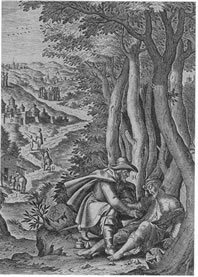
\includegraphics[height=4cm]{../../graphics/samaritan.jpg}
            \end{column}
            \begin{column}{7cm}
                ``For, the ends of a subject who is an end in itself must as far as possible be also my ends, if that representation is to have its full effect in me.'' (G 4:430) 
            \end{column}
        \end{columns}
\end{frame}


\section{Summary}

\begin{frame}<presentation>[label=slide14]
    \frametitle{Summary}
        \begin{columns}
            \begin{column}{3cm}
                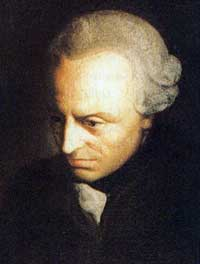
\includegraphics[height=4cm]{../../graphics/kant.jpg}
            \end{column}
            \begin{column}{7cm}
                \begin{itemize}
                    \item Whereas the First Formula specifies the form of the law (its universal applicability), the Second Formula specifies the matter of the law (the substantive value that grounds our duty)
                    \item Appreciating the substantive value that grounds our duty deepens the derivation of our more specific duties
                \end{itemize}
            \end{column}
        \end{columns}
\end{frame}

\end{document}
